\documentclass{article} % For LaTeX2e
\usepackage{url}
\usepackage[
style=authoryear,
backend=bibtex,
]{biblatex}
\usepackage{graphicx}
\graphicspath{ {./Graphics/} }
\usepackage{enumitem}
\usepackage{placeins}
\usepackage{float}

\addbibresource{ProposalBib.bib}

\title{STOR 496 Independent Project Proposal}
\author{
Adam Dameron
}

\begin{document}


\maketitle

\begin{abstract}
This proposal is for a project which seeks to use machine learning and object oriented statistics to model international human trafficking behavior. The goal of this project is to show which aspects of trafficking are most correlated with changes in a nations development. This is for the purposes of informing law enforcement and policy makers of what characteristics to be searching for.
\end{abstract}

\section{Introduction}
	Human trafficking occurs on a global scale, and has been recorded as an international concern since the year 1913 \parencite{Aromaa2007}. Many attempts have been made at defining it, yet these definitions remain unclear and vary greatly. Human trafficking is strongly believed to occur in every country, and victimizes individuals of all ages, genders, and backgrounds \parencite{JacK2012}.\medskip
	
	A major gap in the global understanding of international human trafficking, is in how human trafficking is affected by changes in a country's economic and social development. The United Nations mentions this fact in its "Introduction to Human Trafficking," and describes trafficking as a "multidimensional problem," where a development is applicable \parencite{kangaspunta_2008}. However, there exists very little quantitative analysis into how trafficking and development are connected. Additionally, it has been shown previously that economic and social development has a substantial effect on the migration rates into and out of a country, which in-turn is correlated with human trafficking \parencite{USEconPower, EastEurope}. This research seeks to provide more insight into what connections exist between development and human trafficking, and quantify these relationships in a manner which is easy to interpret.
	
	%Possibly Redundant%
	%Despite mounting global concern, there still exists very little data on the matter of human trafficking, and of the data that does exist, much of it is poorly maintained or incomplete \parencite{Aromaa2007}. Fortunately, there are statistical methods of handling missing data, particularly in the fields of epidemiology, and public health \parencite{abraham_russell_2004}; however, these methods have yet to be applied to data that exists on human trafficking, with the intention of modeling long-term shifts in certain aspects of human trafficking.%
	
\section{Background Information}

The trafficking of humans is a multifaceted problem which exists at all levels from local to international \parencite{Aromaa2007, JacK2012}. The United Nations defines human trafficking as “recruitment, transportation, transfer, harboring or receipt of people through force, fraud or deception, with the aim of exploiting them for profit” \parencite{Raymond2002}. In order to truly understand the scope of this problem, one must begin by gaining an understanding of the different types of trafficking, and the reasons why it is such a widespread issue in all locations; regardless of economic, social, and cultural stability.

\subsection*{Defining Types of Trafficking}

The United States State Department has has a designated "Office To Monitor and Combat Trafficking in Persons" since October of 2001. This office publishes a yearly "Trafficking in Persons Report," and in this report, two types of human trafficking are reported on: sex trafficking, and labor trafficking \parencite{StateDept}.

The U.S. State department defines sex trafficking as
"...activities involved when a trafficker uses force, fraud, or coercion to compel another person to engage in a commercial sex act..." Similarly, labor trafficking is defined as "...activities involved when a trafficker uses force, fraud, or coercion to exploit the labor or services of another person \parencite{StateDept}." Needless to say, these definitions lack depth, and seem vague in nature.

Polaris is a non-profit organization that reports, analyzes, and educates others on the intricacies of human trafficking in the United States. Alternatively to the U.S. State Deparment's two proposed types of human trafficking, Polaris has defined twenty-five different types of human trafficking that are very-much present in the United States. To preface the 80 page report on "The Typology of Modern Slavery," Polaris states: "...the ways humans are exploited differ greatly. Each type has unique strategies for recruiting and controlling victims, and concealing the crime. \parencite{polarisTypology}"

The types of trafficking described by Polaris were based off of over 42,000 reports made to the "Human Trafficking Hotline." The types mentioned range from agricultural work and farming to personal sexual servitude and escort services. However, Polaris notes that most cases of human trafficking will involve more than one type, and even these types may not fit neatly into "sex trafficking" or "labor trafficking" \parencite{polarisTypology}.

In conclusion, there is no neatly defined categories for human trafficking, except the general consensus in academia, law enforcement, and non-profits, seems to be that aside from a few edge cases, most instances of human trafficking unfortunately have to be reduced to being in one of two major categories, as any deviation from this results in inconsistent and contradictory definitions. It is for these reasons that we will attempt to use a different method of classifying human trafficking cases, but is important to recognize the work already done on this topic by powerful entities such as the U.S. Department of State, and a large organization such as Polaris.

\subsection*{United States's Involvement in International Trafficking}

The United States has long been growing into the global economic leader it is today \parencite{USEconPower}. With this increase in global influence comes an increase of international crime within the country's borders. Sex and labor trafficking have both been long-standing issue within the United States. In 2000, the United Nations developed the Palermo Protocols; These protocols sought to "prevent, suppress and punish trafficking in human beings" \parencite{Polermo}. In 2005, the United States ratified the protocols in an effort to fight the increasing prevelance of labor and sex trafficking. 

Despite both labor and sex trafficking being present in the United States, most media and law enforcement attention has specifically been targeted towards sex trafficking, particularly of children \parencite{MediaRep}. Logically we can assume that given the influence the US has on global trade and international crime, that there is are instances of individuals of other citizenships being exploited within the country, and in ways that are not just sex trafficking.

\FloatBarrier

\begin{figure}[H]
	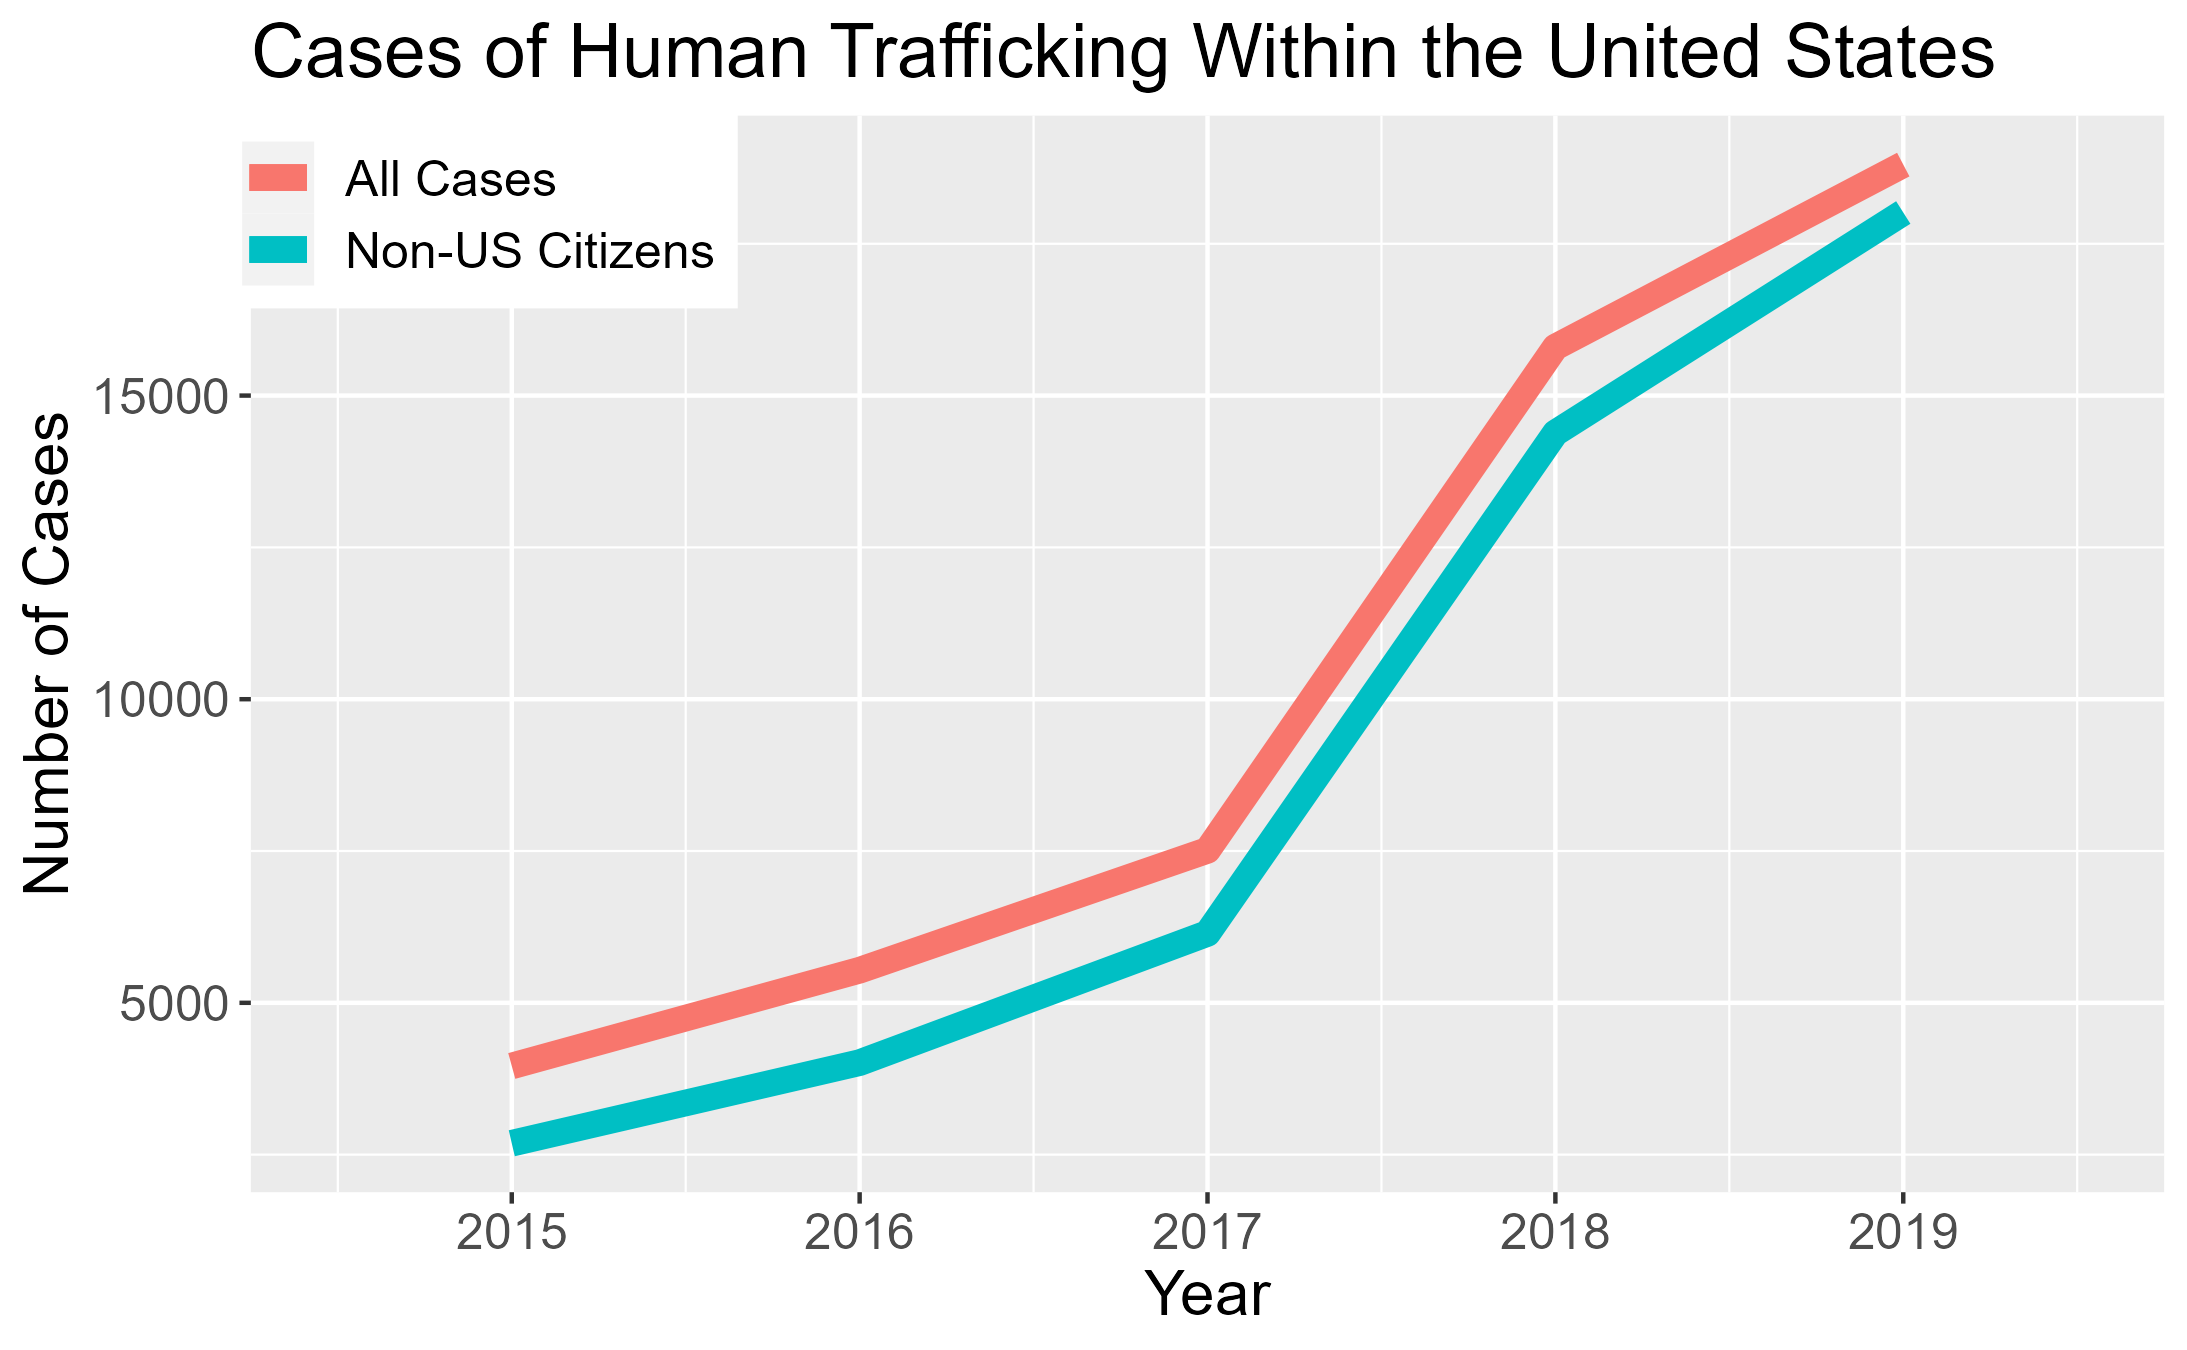
\includegraphics[width = \textwidth]{USTrafficking}
	\scriptsize{\caption{Created with data from \cite{CTDC}}}
\end{figure}

\FloatBarrier

As evidenced in this simple chart, in a span of only 4 years, the number of cases in the United States alone has nearly quadrupled. Although, it is important to note that this is likely to be a severe under-counting of the true number of human trafficking victims each year. Even so, having roughly 20,000 cases in 2019 alone is rather extreme, and shows that this is very much an issue that exists in the United States. Of additional importance is the fact that a large proportion of all cases in the US are ones involving non-US citizens. This means that not only is trafficking present in the US, but international trafficking is of major concern.

\FloatBarrier

\begin{figure}[H]
	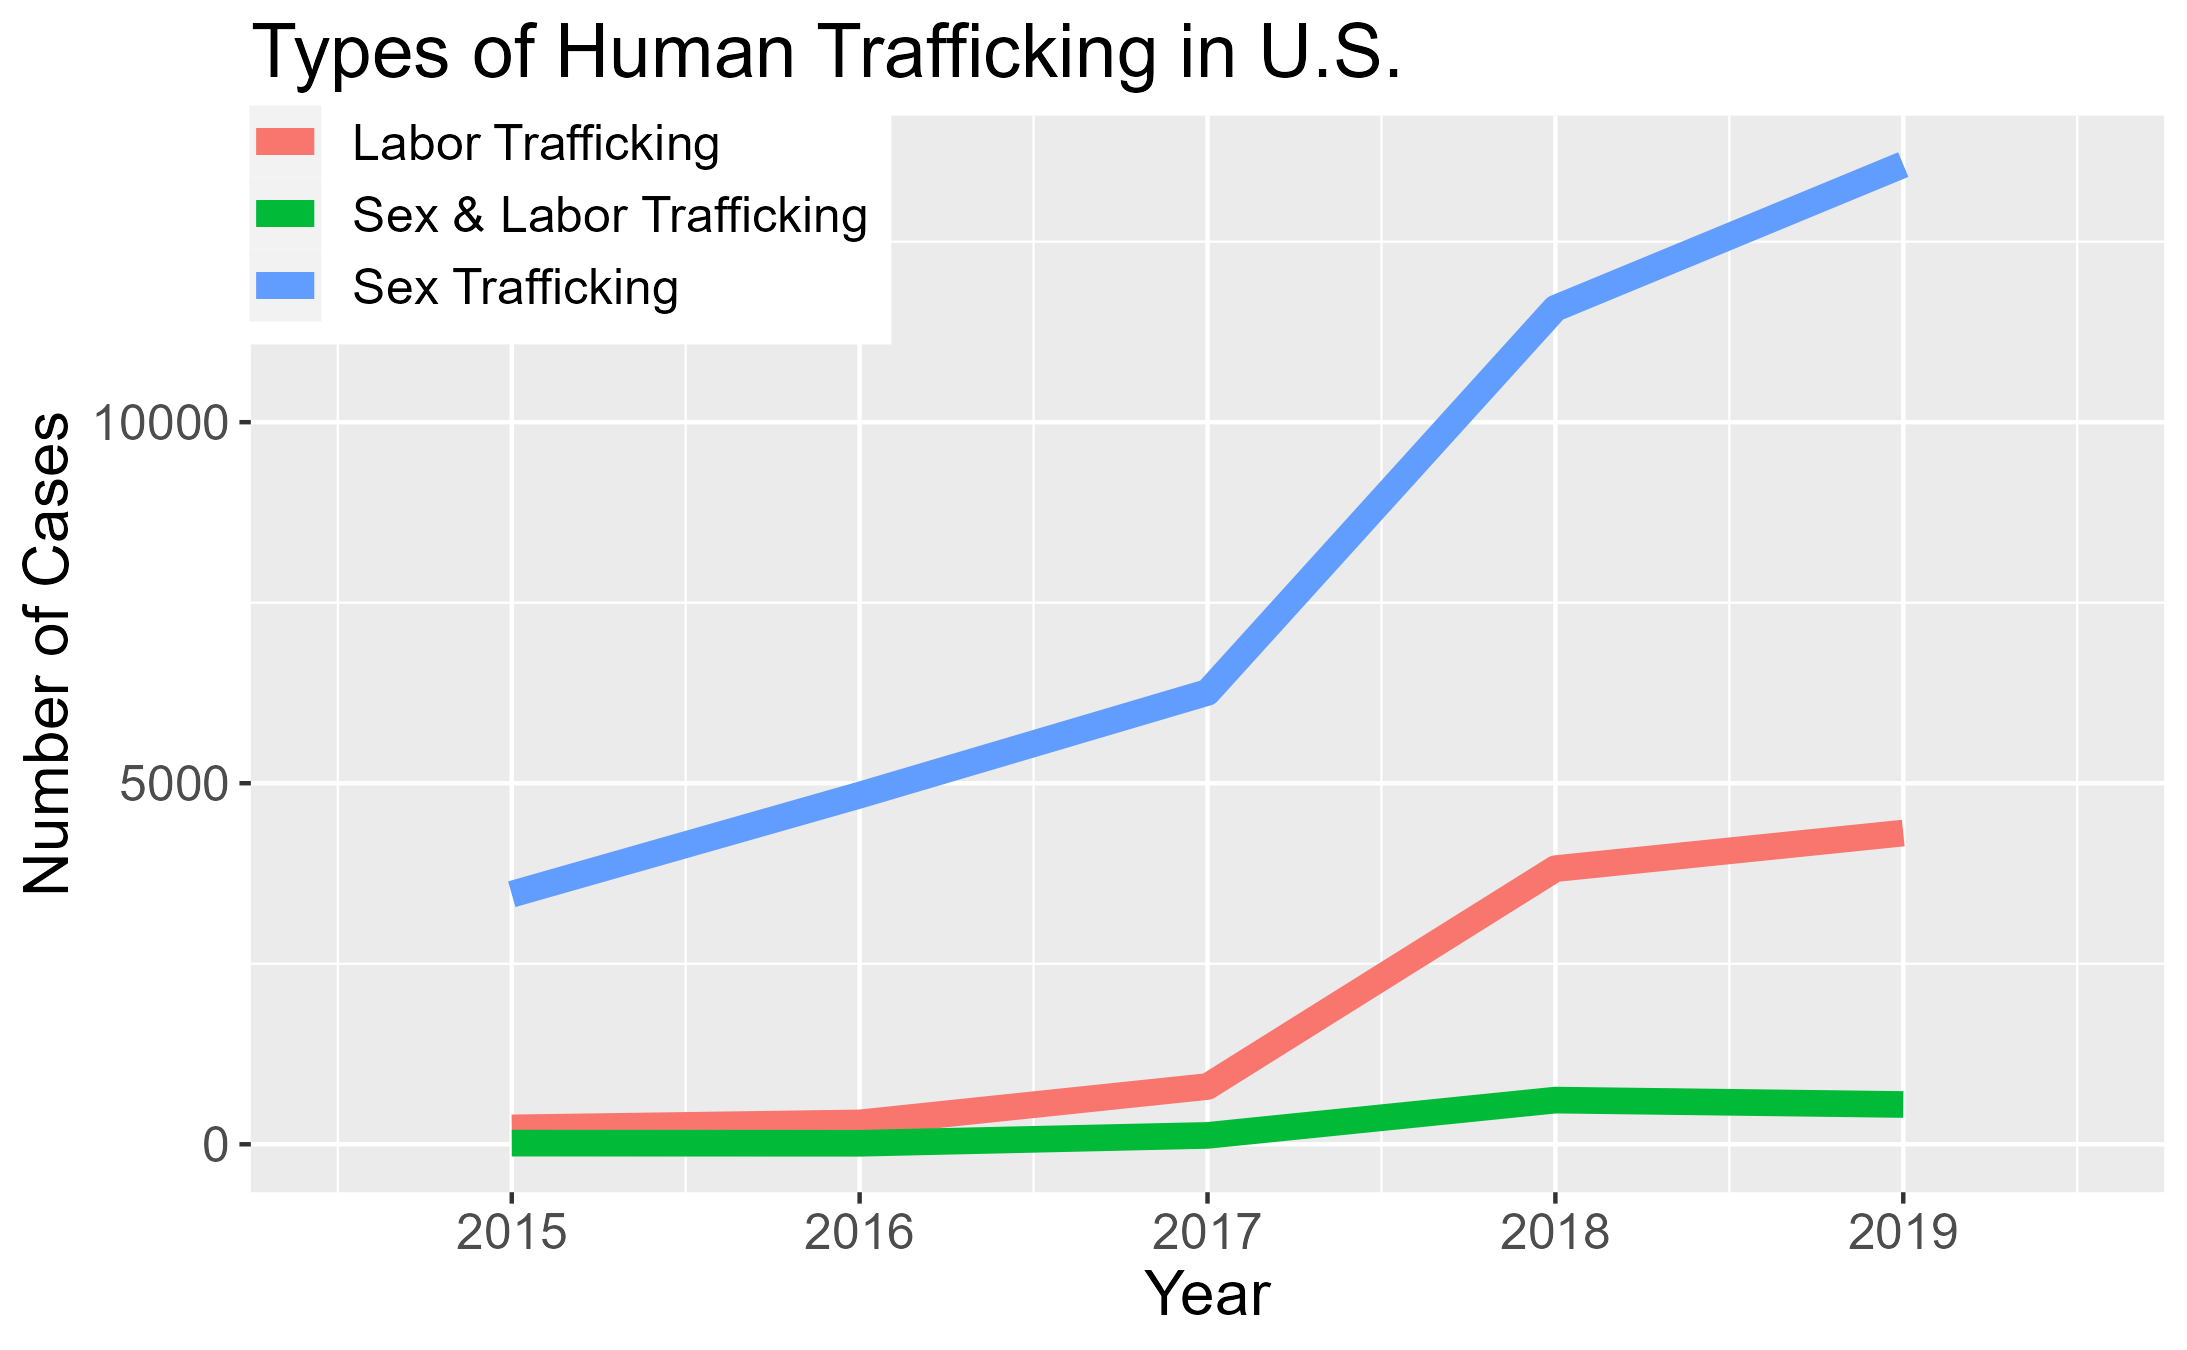
\includegraphics[width = \textwidth]{USTrafficking2}
	\scriptsize{\caption{Created with data from \cite{CTDC}}}
\end{figure}

\FloatBarrier

From this plot, one can see that again, each year there is an increase in the total number of reported cases; however, we see that a significant number of cases exist in which sex trafficking is not the sole type of trafficking present. Thus, even within th U.S., international trafficking is a very real issue, and it exists in all forms, not just sexual. Thus it would be beneficial to better understand, or even predict, what aspects of these victims law enforcement should be knowledgeable of. 

\subsection*{Scale of International Trafficking}

It is difficult to put into words the scale of international human trafficking. However, by looking at the number of human trafficking victims reported in each country, and then determining what percent of them are from other countries, we can visualize the scale of the problem.

\FloatBarrier

\begin{center}
	\begin{figure}[H]
		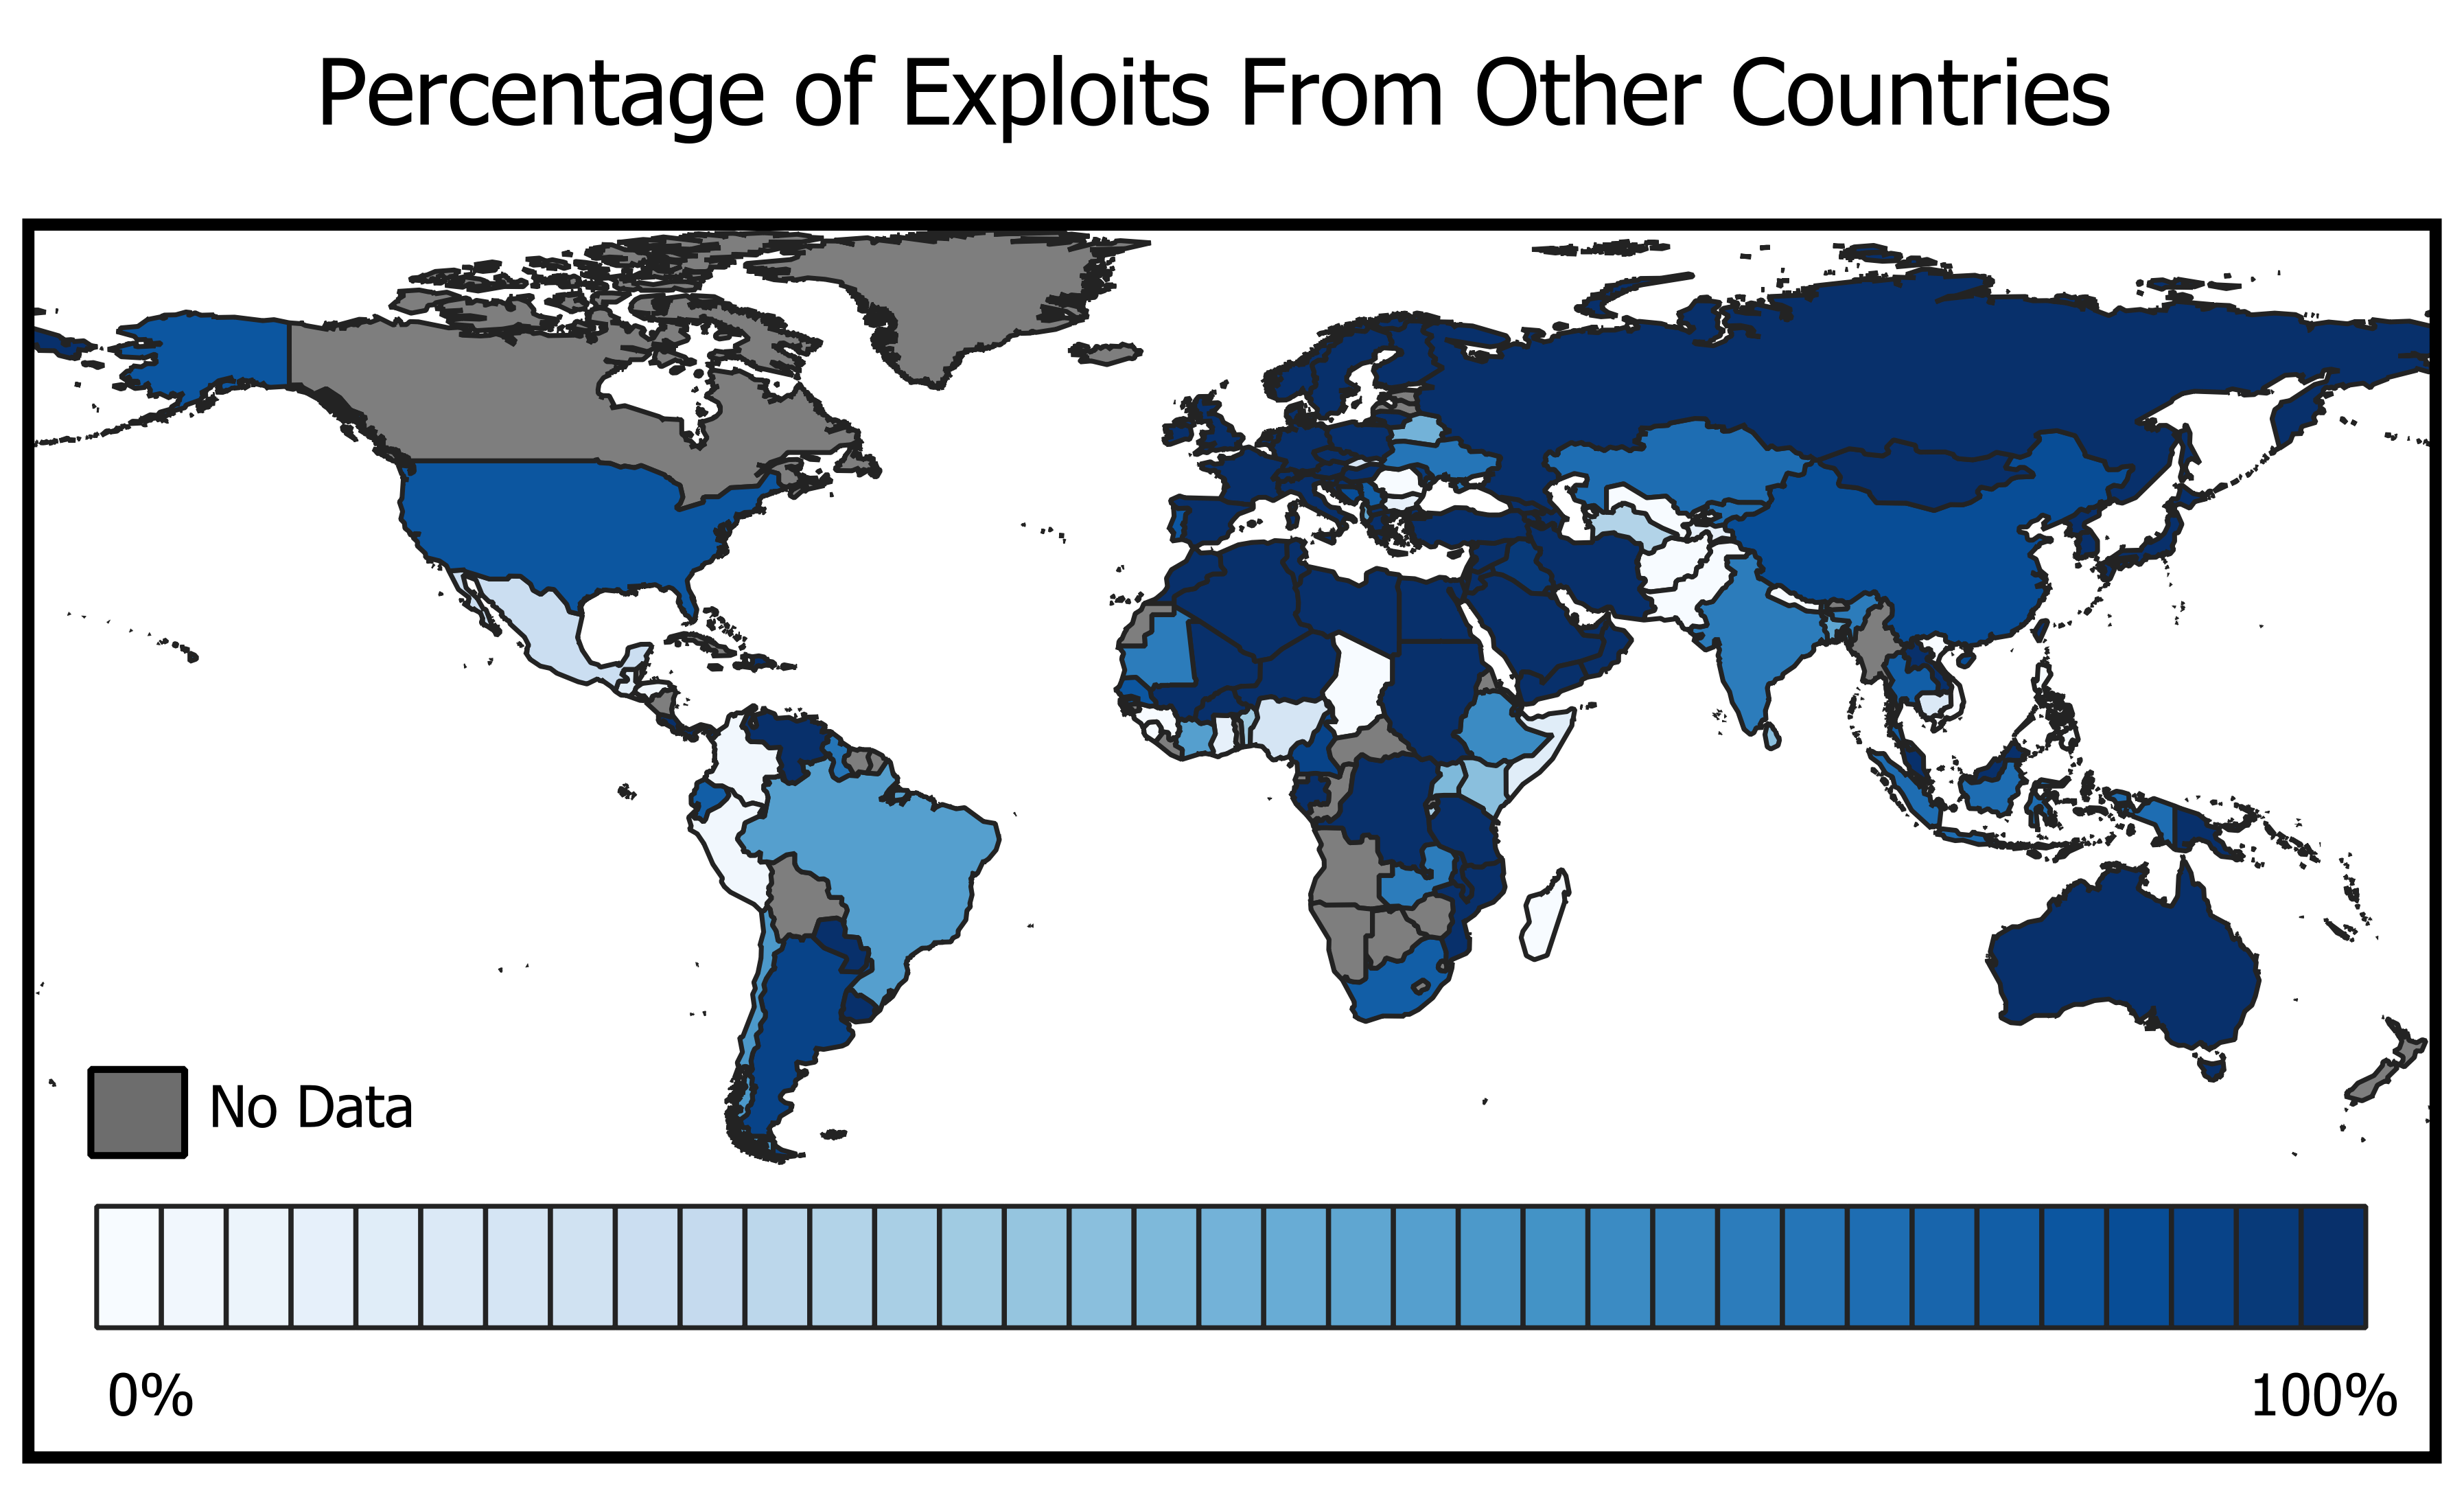
\includegraphics[width = 5.6in]{ProposalMap1}
		\scriptsize{\caption{Created with data from \cite{CTDC}}}
	\end{figure}
\end{center}
\FloatBarrier

In this map, each country is colored one of many shades of blue, where darker shades correspond to a higher percentage of international victims within the country. We can see in the map that there are a lot of dark-blue regions. Some distinctly blue regions are North-Africa and Europe. There are also some scattered regions in South-East Asia which have a high percentage of international trafficking victims. 

Of additional interest are the very light-blue or even white regions of the map. these regions have a low percentage of international trafficking victims, which means that these countries almost exclusively have victims who originate from within the country. While this visualization gives us an idea of the prevalence of international victims who are exploited in each country, it does not show us how many victims originating from a country are "exported" to other regions.

\FloatBarrier

\begin{center}
	\begin{figure}[H]
		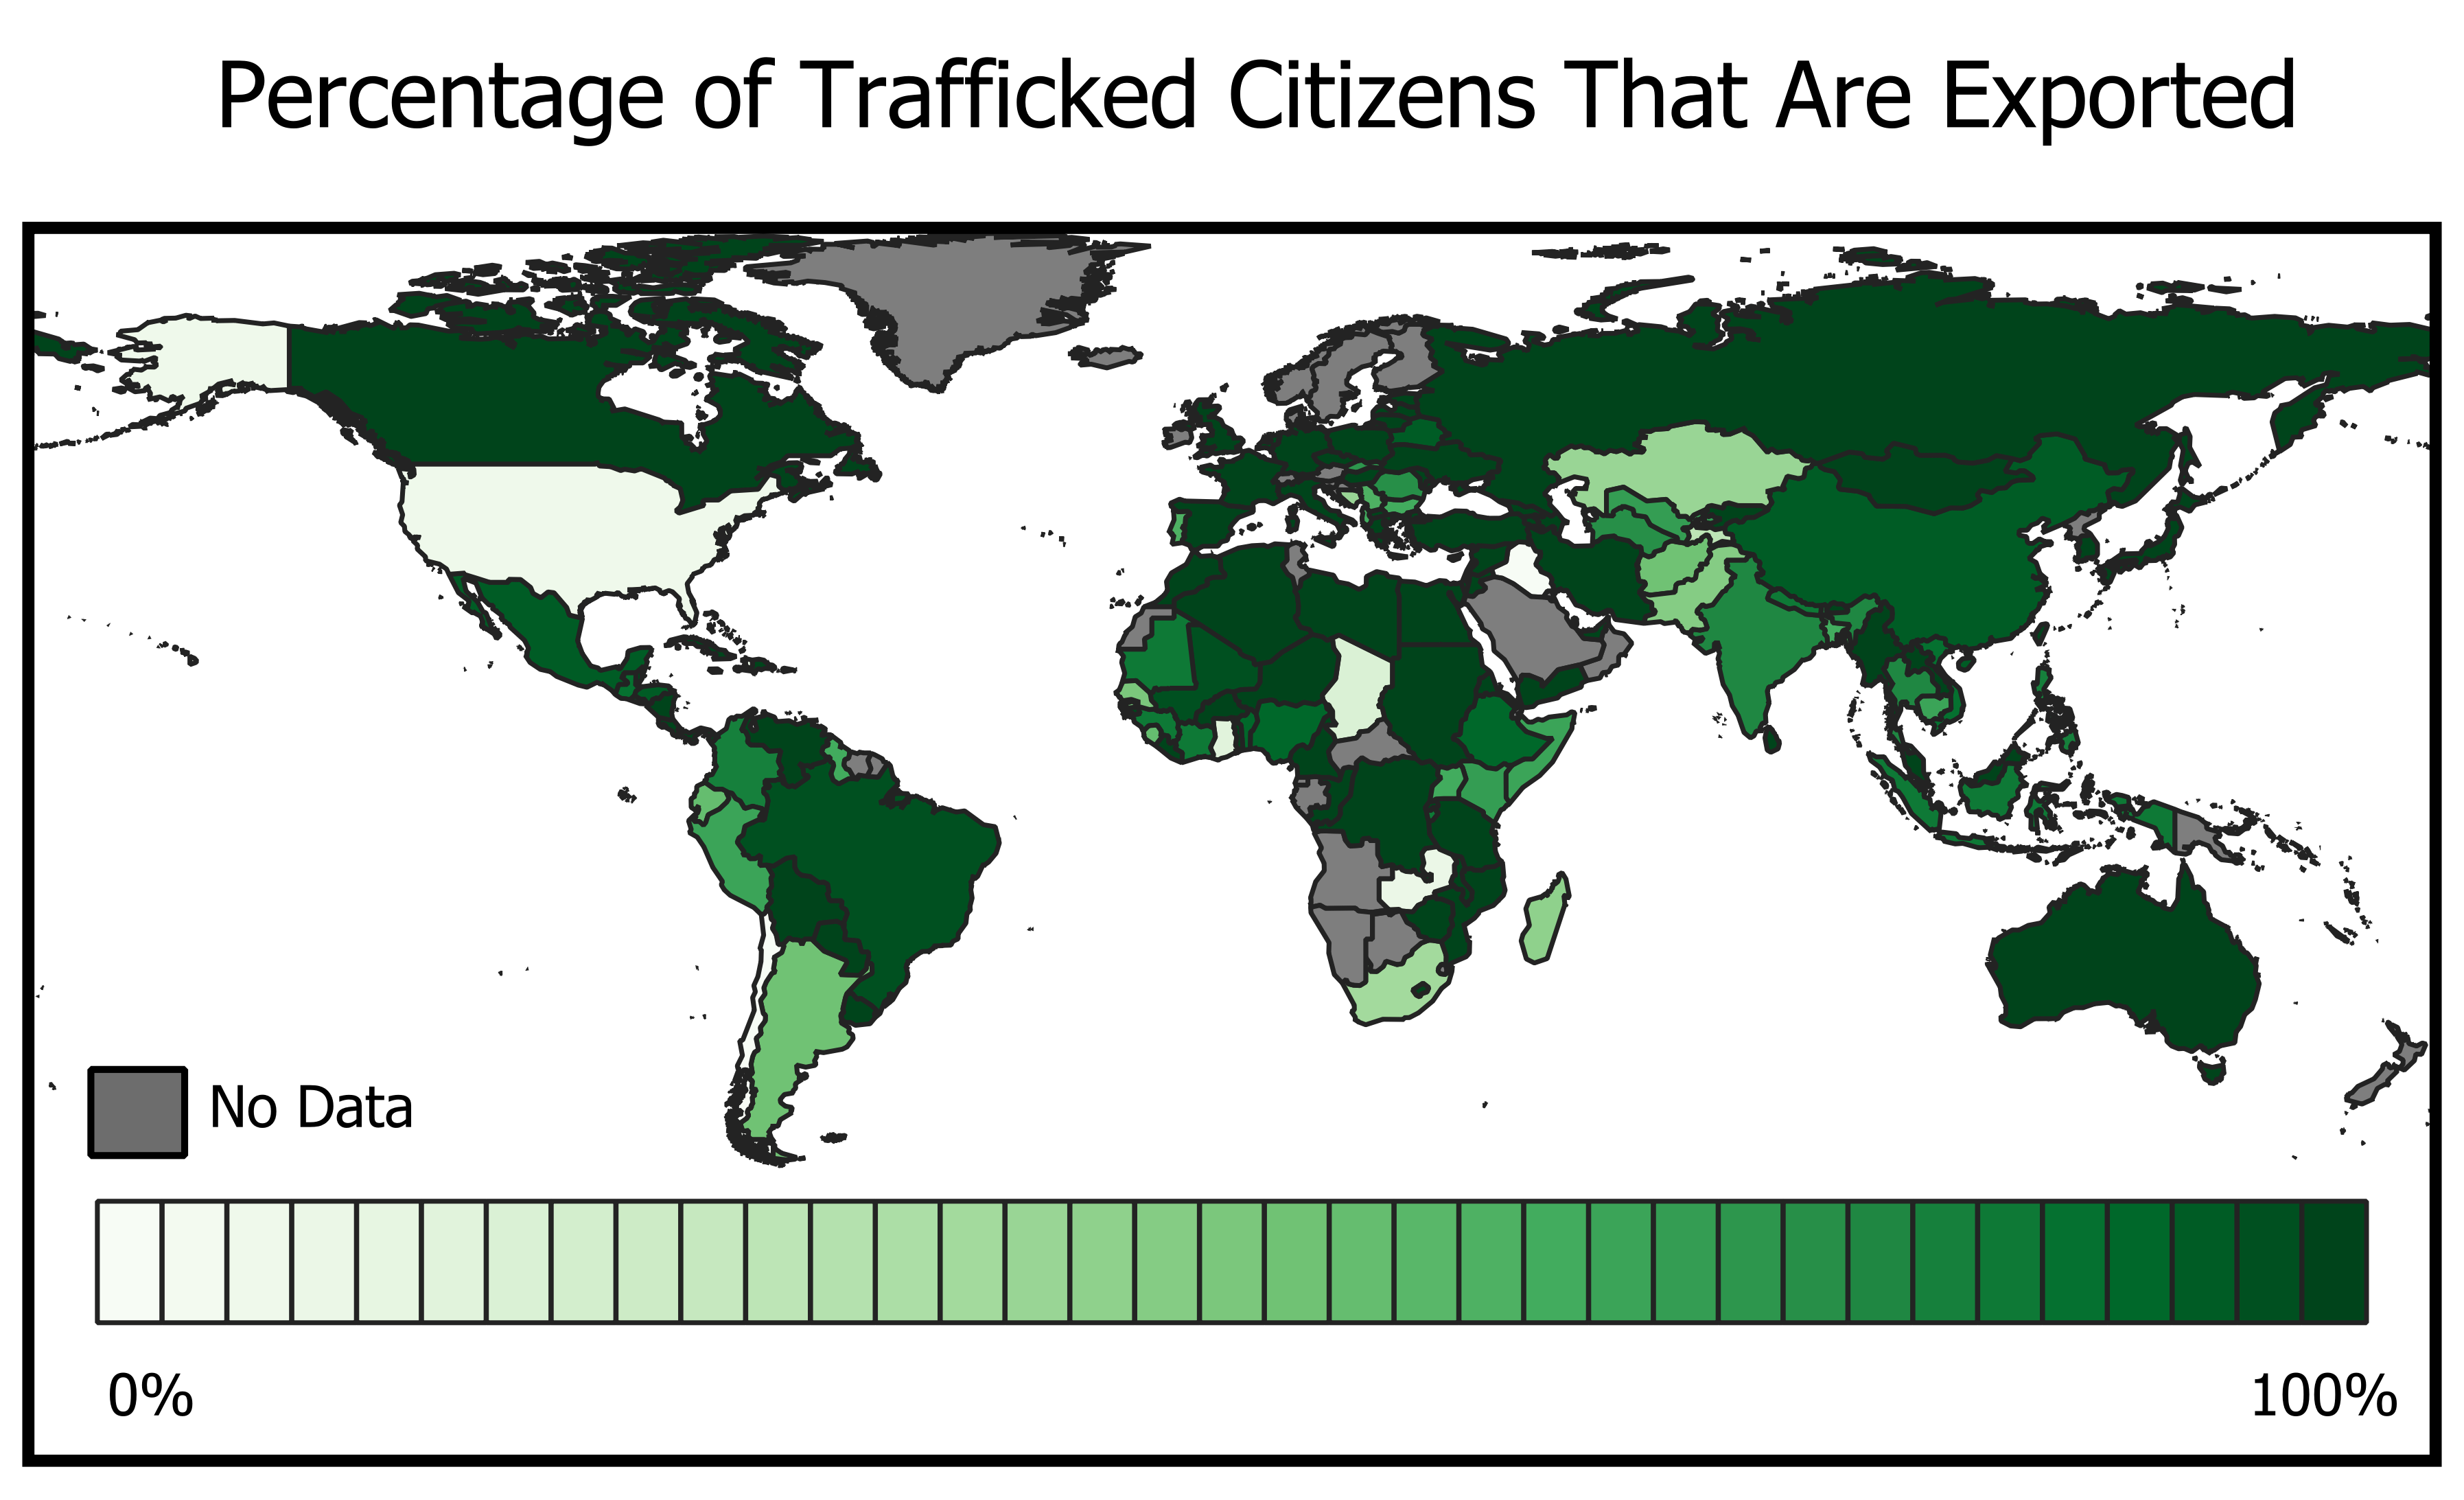
\includegraphics[width = 5.6in]{ProposalMap2}
		\scriptsize{\caption{Created with data from \cite{CTDC}}}
	\end{figure}
\end{center}
\FloatBarrier

This map is similar to the first one in that a darker color (in this case green), indicates a higher percentage of trafficked citizens who are exported from their country of origin. These two maps on their own do not paint a good picture, but when viewed together, they provide useful qualitative information.

Some preliminary conclusions one could make from these maps. For example: Mexico has a low percentage of victims from other countries, and a large percentage of Mexican citizens who are exploited, exploited in other countries. Thus we can conclude that Mexico is an "exporter" of human trafficking victims.
	
The Northern region of Africa has a high percentage of citizens that are exported, as well as a large percentage of exploits which are from other countries. This means that countries in the region displace many of their exploited citizens to other countries, but bring in victims from other countries. This suggests that individuals in North Africa are trafficked to other regions to fill a certain "role," and victims from other regions ar imported to fill a different role. In fact, we know this to be true as a result of previous studies on the region.

The smuggling of migrants and laborers from Northern Africa to Europe explains the high percenage of exploited citizens that are exported \parencite{AfricaExport}. The high percentage of victims within these countries coming from other regions is explained by the trafficking of individuals from West Africa to North Africa. Many West African migrants attempting o get to the Mediterranean Sea, are often intercepted and trafficked along their route through Algeria and Libya \parencite{AfricaImport}.

Mexico and North-Africa are just two examples of the many types of qualitative conclusions one can make from these maps; however, a major question these maps could never answer is what types of trafficking are present, what indicators exist to determine the typology of trafficking victims in a region, and most importantly, how the stage in development of a country effects these indicators and types of trafficking.


\section{Prior Research}

%A Step Towards Modeling and Destabilizing Human Trafficking

In 2010, Shreya Amin writes "Knowledge about the structure of a human trafficking network, from beginning of the process to the end, is extremely important and is missing.\parencite{firstML}" This was at the end of her paper exploring the potential of using machine learning to model human trafficking. In her research, she explored the large amounts of data involved in human trafficking and mentions the ways in which machine learning can be applied. Amin's research is the earliest example I could find of research being conducted on the potential of applying machine learning to solve the issue of human trafficking. An important fact to note is that she makes no mention or references to other research that specifically attempts to use machine learning on this specific problem. This is evidence of her being the first person to publish this idea.



%Human Trafficking: A Perfect Storm of Contributing Factors

In \emph{Human Trafficking: A Perfect Storm of Contributing Factors} \parencite{SlaveBook} a connection is theorized between human trafficking and the Demographic Transition Model. The author, Susan Tiano, talks about how the rise and fall in birth and death rates has an effect on human trafficking. By first talking about the growth of the "underground economy" in relation to shiftas in Demographic Transition, Tiano sets the stage to infer that trafficking is no different. Tiano's research further validates the claim that Demographic Transition does have an effect on human trafficking, but Tiano was unable to quantify such a relation. Thus, being able to quantify these relationships would fill a major gap in the current knowledge of the human trafficking landscape.

%The Use of Bayesian Networks for Realist Evaluation of Complex Interventions

\emph{The Use of Bayesian Networks for Realist Evaluation of Complex Interventions} \parencite{Bayesian} applied Bayesian Networks, a statistical modeling technique, to outline the interactions between variables related to labor trafficking. The authors of this paper paper used many of the same predictors that will be used in my proposed research. Variables such as how the victim was recruited, the age of the victim, and whether or not the victim was exploited for physical labor, are also present in The CTDC Dataset. Additionally, this Bayesian Network uses variables such as caste (location in a social hierarchy), education level, and literacy. These variables are important because they have been shown to correlate highly with the stage of development of ones country. For example, countries with lower stages of development, will typically have lower literacy rates. 

One interesting finding, which is outlined in the paper's conclusion, is the conclusion that "changes to the variable \emph{destination} have the largest influence on the outcomes,\parencite{Bayesian}" meaning that it was determined in this study that the destination country of a trafficking victim had the largest effect on whether or not an individual was a victim of labor trafficking. Thus, this study gives some evidence to support the hypothesis that the stage of a development of a country would have a significant effect on the typology of victims within that country.



%Potential Impact of Climate Change on Human Trafficking

In \emph{Potential Impact of Climate Change on Human Trafficking} \parencite{Climate}, there is discussion of many of the direct and indirect effects that climate change has on international human trafficking. Of high interest in this article is what is said about human trafficking in the United States, in the aftermath of Hurricane Katrina. According to this article, the Federal Government temporarily removed certain worker protections in the New Orleans area after the hurricane. This led to a huge influx of labor trafficking victims into the region in order to help rebuild. This plainly demonstrates that labor trafficking can be used to fill a sudden demand for cheap labor \parencite{Climate}. It also is an example of the major, somewhat instantaneous effect that federal governmental legislation can have on the typology of trafficking within their borders. Thus, making informed lawmaking decisions is vitally important in preventing human trafficking.

In the case of Hurricane Katrina, the Gulf Region essentially became less developed than the rest of the United States, and as a result, labor trafficking spiked \parencite{Climate}. This is yet another example of the effect that development can have on trafficking in a region.

%The Economics of Human Trafficking and Labour Migration: Micro-Evidence from Eastern Europe.

\emph{The Economics of Human Trafficking and Labour Migration: Micro-Evidence from Eastern Europe}\parencite{EastEurope} takes an in depth look at human trafficking in Eastern Europe, and takes the time to discuss the qualitative relationships between country development and trafficking. This article provides examples of the supply and demand aspect of trafficking, and how it relates to development in Eastern European countries. The research determined that poorer, less developed countries experienced more "out-migration" than countries that were more developed \parencite{EastEurope}. This helps to reinforce the hypothesis that development does have an impact on whether a country fulfills a supply or demand role in the global human trafficking nexus. Additionally, this research assumes a homogeneity throughout a country, which is not an ideal assumption to make; however, this is more in line with the assumptions made in my research and thus this article is a good comparison to make with my own ideas.


\section{Objective}

The Global K-Anonymized Dataset (CTDC Dataset) is a dataset which was developed and is maintained by the International Organization for Migration (IOM). This dataset was created with the aim of providing a large centralized database of human trafficking cases all over the world. This dataset contains over 150 thousand entries, and has data from 189 countries. This collection of data exists publicly, and each entry has been ''anonymized'' in order to protect the identities of the victims.

The CTDC dataset was initially created to solve the problem of human trafficking databases being inconsistent, and unreliable. By creating this dataset, IOM created a database which is easy to use and navigate. The creation of this dqataset has solved a major issue of quality data analysis on human trafficking being impractical, or even impossible.

The objective of this research is to use the CTDC dataset, to develop models that show what types and indicators of trafficking are present in countries of different stages of development. This is a significant gap in the existing knowledge offered to law enforcement and law makers in regards to international human trafficking. By creating these models, it will provide these entities with information more specific to the country they serve, and will allow them to make more informed decisions.

Some of the specific models that will be explored are a binary classification into "High Development" and "Low Development" countries. This binary classification would be accomplished with logistic regression, in which each predictor has a calculated value that shows how big of a connection it has with being high or low development. 

This could then be scaled up to a multinomial model in which each variable has a calculated value of how much a change in the variable value, will effect the probability of being a victim in any of the stages of development. For example, the model could determine that given a victim is male, the probability of being in a stage 4 country increases, but the probability of being in a stage 3 country decreases. By looking at these values, combined with P-Values, we can conclude which variables have the greatest relationship with stage of development.

\section{Preliminary Reasoning and Analysis}

The Counter Trafficking Data Collaborative (CTDC) has a publicly available, anonymized dataset, which is a collection of over 400,000 entries for human trafficking victims \parencite{CTDC}. The database has plenty of useful information, such as country of citizenship, country of exploitation, and many variables expressing the type(s) of trafficking the victim experienced. This data set is what this research and models will be based on, as it is the largest publicly available database for instances of international human trafficking.

While the CTDC database is extremely large, it does not contain information on a country's development. For this, one needs a numerical way to categorize countries into "stages," as the goal is to make a generalized model for stages of development, not one that pertains to specific countries. One way to categorize countries would be by using the Demographic Transition Model \parencite{bongaarts2009}. Using this model, a country can be categorized into one of 5 stages, with stage 1 being the lowest developed countries, and stage 5 being the most developed.

Unlike many other ways of classifying countries in terms of their development, this model uses birth, death, and migration rates to determine a country's stage \parencite{bongaarts2009}. While these rates are not directly related to a country's economic growth or decline, the model has been shown to be very successful at expressing economic changes, while not being as strongly influenced by sudden, temporary economic setbacks or "booms" \parencite{kirk1996,bar2010,galor2000}. The model has even been shown to help predict changes in the "shadow economy," in areas of illegal activity such as drug trafficking \parencite{sch1994}. It is for these reasons that I believe there exists a way to efficiently model and predict changes in the human trafficking typology of a country as it becomes more or less developed.

For our data, a complete entry is a case in which we have a value for all variables in the dataset. An incomplete entry is any entry in which there are values which are unknown, such as the age of the victim, or the type of trafficking experienced. By looking at complete entries in the CTDC Dataset, we can do a preliminary correlation comparison. We can take both the stage of the citizenship country, and exploitation country for a victim, and see if this correlates with any aspects of trafficking they experienced. The closer to perfectly correlated (-1 or 1) or connected two variables are, the more red or blue the circle will be. If a circle is red, that means the trait is seen more in low stage countries, and if it is blue, it is observed more often in high-stage countries.

\hspace*{-1.5cm}
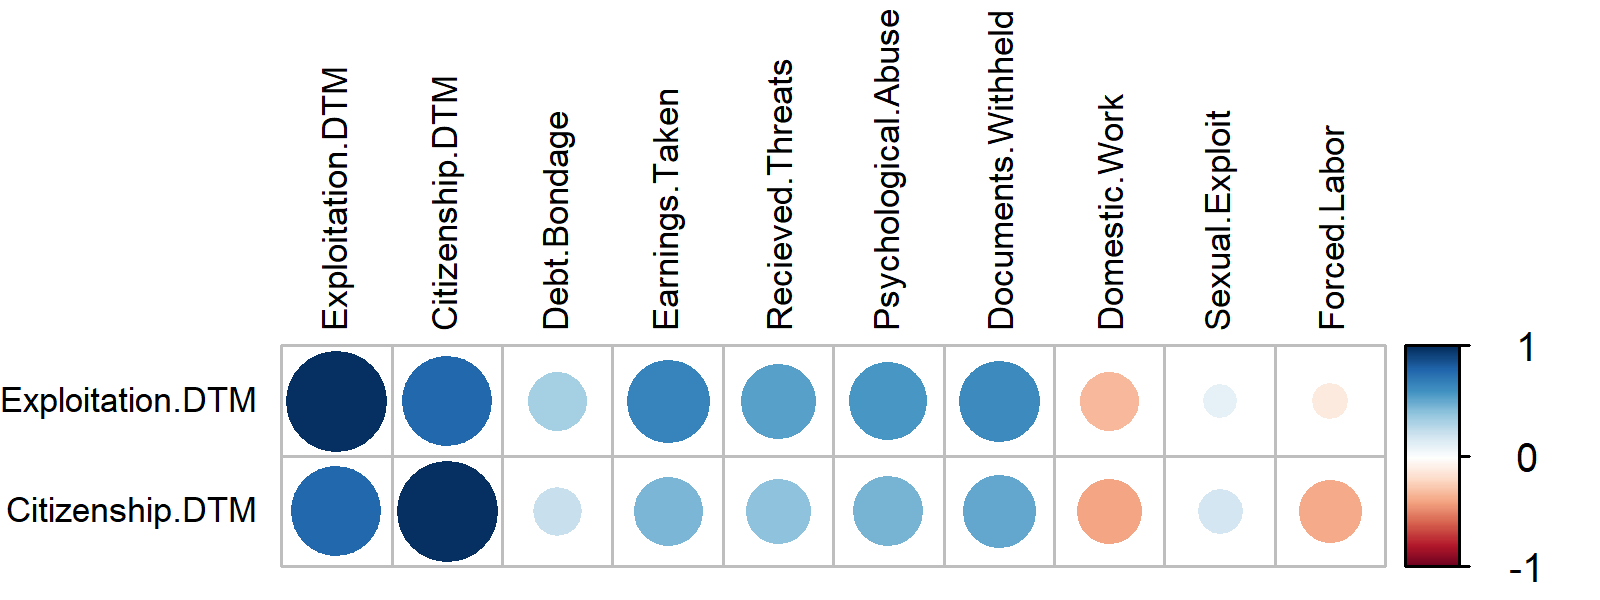
\includegraphics{Corrplot} \bigskip

Each of the variables included in the plot have at least a moderate correlation with DTM. As such, it would be beneficial to further quantify and model what types of relationships do exist within the data.


\section{Research Plan}

The eventual goal of this research is to create a multinomial regression model. This is a probabilistic model which, for any given observation, it will give the probability of the observation being in a certain group. In our case, the groups will be the stage of development of a country in which a human trafficking victim is found. By creating a model of this type, we can determine which aspects of human trafficking have the greatest correlation with the stage of development of the country. As a result, one can learn what impact a change in the level of development within a country has on the typology of human trafficking. Thus, we can quantify just how much of an effect country development has on human trafficking.

The creation of this model will initially be done using a multinomial neural-network architecture to find which coefficients for predictors provide the least number of classifications on the data. If time permits, other model architectures will be tested to see if any of those perform better on our data set.


Perhaps the biggest hurdle to be overcome is the sheer lack of complete entries in the data set. As a result, the first steps of this research will involve analyzing what data is missing, and determining how to address that. By using visualizations and quantitative measurements, we can determine which observed values (predictors) are causing the most incomplete entries in our data. We can also determine which predictors are missing in tandem, and which ones are missing independently. By doing this, we can determine which variables we should remove first, and see if it gives us enough complete observations to create a helpful model.

To test the effectiveness of our model, we will randomly split our data into two groups: a group for training the model, and a group for testing the model. After training the model, we will simply input the observations for the test set, and see how accurately the model is able to classify the observations.

\subsection{Assumptions and Limitations}


For the purposes of this research, instead of classifying an instance of human trafficking into one type or category, we will use many different categories to describe a case in the following way. We will begin by having two main categories with sub-categories. Then for each case, we will "classify" it by simply observing which of the sub categories are present. If all of the observed sub-categories fall under sex trafficking, then we can classify the case under sex trafficking. Similarly the same would happen with labor trafficking, and if a case has aspects of both, then we classify the case as "labor and sex trafficking".

\FloatBarrier
\begin{table}[htb]
	\begin{tabular}{ |p{3cm}|p{3cm}||p{3cm}|p{3cm}|  }
		\hline
		\multicolumn{4}{|c|}{Types of Human Trafficking}                                 \\ \hline
		\multicolumn{2}{|c||}{Sex Trafficking} & \multicolumn{2}{|c|}{Labor Trafficking} \\ \hline
		Prostitution    & Private Services     & Agriculture        & Aquafarming        \\
		Remote Services & Pornography          & Begging            & Construction       \\
		&                      & Domestic Work      & Hospitality        \\
		&                      & Illicit Activities & Manufacturing      \\
		&                      & Mining or Drilling & Peddling           \\
		&                      & Transportation     &                    \\ \hline
	\end{tabular}
	\caption{Types of Human Trafficking with Sub-Categories}
\end{table}
\FloatBarrier

Each example in our sub-categories, have a binary variable in the CTDC Dataset. this means that for a sub-category, the entry has a value of 0 if it is not observed, and 1 if it is. These values could also be missing, and if we determine that a variable is missing very frequently, then it may be worth removing that variable for all entries in order to have a more complete dataset. For example, if it is determined that a large percentage of entries have no entries for "Mining or Drilling," then we may remove the variable from the dataset entirely in order to create a more robust model.


\section{Final Goals}

One explanation for why law enforcement is unequipped to adequately address human trafficking is that they "[do] not have the time,
resources or expertise to address [the] problem," \parencite{LawResponse}. The goal of this research is to produce an understanding of the types of connections that exist between certain aspects of human trafficking and how developed an area is. This would allow policy makers to create policies which allow law enforcement to be more equipped to find victims of human trafficking as their country becomes more developed. Importantly, countries can also become less developed, as is the case in countries with civil unrest and that have been effected by natural disasters \parencite{bar2010}. It is vitally important for the leaders of a country to be knowledgeable of the effects these events can have on the human trafficking that exists within their country, such that they are better able to protect and save the victims.


\printbibliography


\end{document}
